\chapter{Hardware}

\begin{figure}[h!]
  \centering 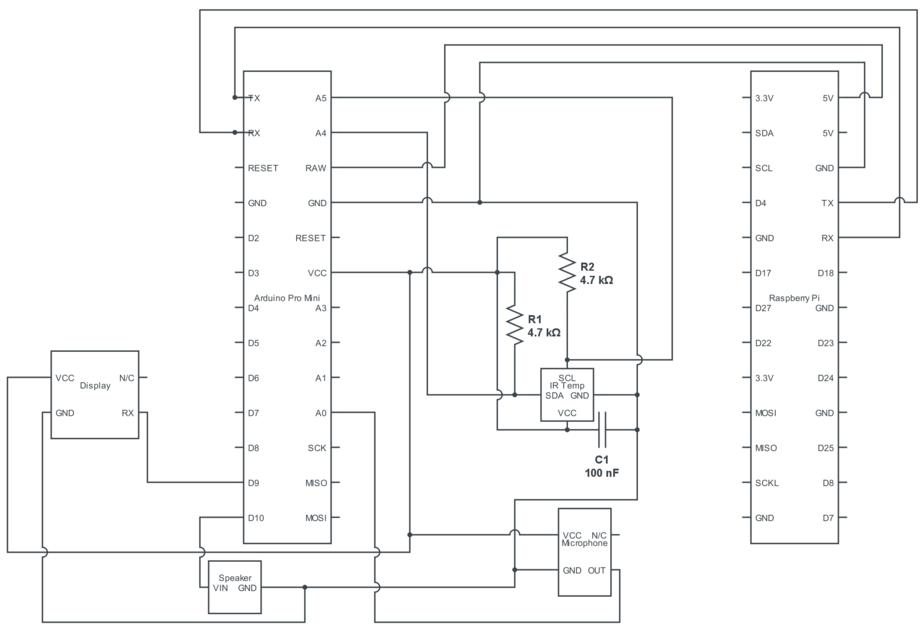
\includegraphics[width=1\textwidth]{schem}
  \caption{Schematic for Impetus.}
\end{figure}

Impetus is comprised of two large components that communicate serially
with each other, with small components (sensors, actuators)
communicating with one of the large components.

\section{Large Components}
\subsection{Arduino Pro Mini}
The Arduino Pro Mini used in Impetus is responsible for communicating
with all the sensors and actuators involved in the device. While most
of the communication is done serially, some sensors and actuators have
single-pin digital or analog interfaces as well.

The model used in this device has an operating voltage of 3.3V with an
8MHz Atmega328 microcontroller.

\subsection{Raspberry Pi}
The Raspberry Pi mainly communicates state transitions to the Arduino
Pro Mini while receiving data from sensors connected to the Arduino to
process and send through Twitter.

The model used is a Model B, Revision 2, with 512MB memory and a 700MHz
ARM processor. Logic voltage is 3.3V, allowing the Raspberry Pi to
communicate with the Arduino Pro Mini without a level shifter.

\begin{figure}[h!]
  \centering 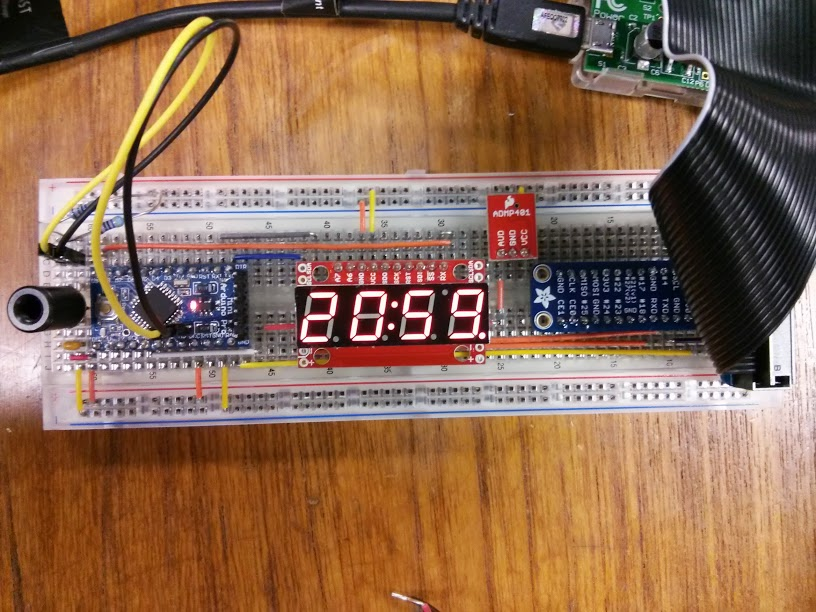
\includegraphics[width=0.75\textwidth]{bb}
  \caption{Components of Impetus (sans Mini Buzzer).}
\end{figure}

\section{Sensors}
\subsection{MLX90614ESF-BCF IR Thermometer}
The Melexis MLX90614 family of IR thermometers measure the surface
temperature of objects that are a distance away from the sensor. It
stores the result in RAM to be accessed through either a PWM or
I\textsuperscript{2}C interface. Impetus communicates with this sensor
through I\textsuperscript{2}C, getting both the object temperature and
the ambient temperature for presence detection.

This particular model (BCF) operates at a voltage of 3.3V, and has a
field of vision of 10\degree, which allows the device to get decent
measurements from objects as large as the human head from roughly 5
feet away from the sensor with minor degradation of accuracy due to
distance.

\subsection{ADMP401 MEMS Microphone}
This microphone is powered at 3.3V and outputs an analog, oscillating
wave from 0V to 3.3V portraying an (amplified) sound wave. In this
device, sound is sampled continuously for very short intervals on
every state cycle in order find the lowest and highest peaks, which
determine volume at that particular interval of time.

\section{Actuators}
\subsection{7-Segment Serial Display}
The 7-segment display is on a breakout board with an Atmega328 which
facilitates serial communication with the device through multiple
serial interfaces. In Impetus, this actuator communicates over one TTL
line (receiving input, never transmitting output) with the Arduino Pro
Mini. Simple commands are sent to it to display time and give some
form of indication as to which state the device is in. This, along
with every other sensor and actuator, operates at 3.3V.

\subsection{Mini Buzzer}
This speaker operates at 3V\textsubscript{DC} with a sound pressure
level around 75dB at 20cm. It is toggled on and off by the Arduino Pro
Mini during the alarm state, and is off for any ofther state.
